\chapter{Metodologia}

Assim como foi discutido no capítulo anterior, para obter os parâmetros de caracterização da acústica interna de dutos circulares com escoamento, é preciso de um modelo que suporte a interação fluxo de massa e variação de pressão. Portanto modelos baseados em métodos de fluido dinâmica computacional se mostram adequados, principalmente aqueles baseados no método de \textit{lattice} Boltzmann assim como foi mostrado anteriormente nos trabalhos de \citeonline{da2006lattice} e \citeonline{da2009sound}. Nesse sentido, há traballhos que validam, aplicam e desenvolvem metodologias de \textit{lattice} Boltzmann no campo de estudo da aeroacústica.

Um desses estudos é o de \citeonline{crouse2006fundamental}, que mostraram a eficácia do método de \textit{lattice} Boltzmann em recuperar as equações de Navier-Stokes de transiente, compressível e viscosa. Há de se ressaltar que validaram também o modelo numérico de um ressonador de Helmholtz com um modelo experimental do mesmo, demonstrando assim a viabilidade da aplicação para problemas de acústica.

No que se trata de desenvolvimento de ferramentas auxiliares para tratar problemas acústicos, \citeonline{kam2006non} desenvolveu uma condição de contorno que caracteriza dissipação de energia acústica e fluido dinâmica, ou seja, uma condição de contorno anecóica. Ela se baseia no acoplamento de mais um termo na equação de Boltzmann para gerar uma região de amortecimento, redirecionando os valores de densidade e velocidade das partículas para um valor alvo, que seria no caso valores médios de densidade e velocidade num fluido em repouso.

\citeonline{marie2009} analisou e comparou esquemas de alta ordem das equações de Navier-Stokes linearizadas com o método de \textit{lattice} Boltzmann. O objeto de estudo para comparação foi análises de dispersão e dissipação de ondas acústicas em regime isotérmico. Conclui-se com esse trabalho que para um determinado erro de dispersão o método de \textit{lattice} Boltzmann se comportou como mais rápido.

No que diz respeito a aplicação do método de \textit{lattice} Boltzmann num problema de aeroacústica, \citeonline{lew2010noise} desenvolveram um modelo numérico em 3D para predição de ruído em um jato turbulento subsônico. Como validação os resultados foram comparados com resultados experimentais e cálculos numéricos feitos a base de \textit{Large} \textit{Eddy} \textit{Simulation} (LES)\abreviatura{LES}{\textit{Large} \textit{Eddy} \textit{Simulation}}. Esse estudo demonstrou as principais vantagens de se trabalhar com o método de \textit{lattice} Boltzmann como por exemplo o baixo custo computacional e a facilidade em inserir \textit{nozzles} com formas complexas no domínio computacional.

Também na área de aeroacústica computacional, o trabalho de \citeonline{shi2013lattice} propõe um modelo em \textit{lattice} Boltzmann para obter dados de diretividade da radiação sonora num duto circular submetido a escoamento subsônico. Os resultados de diretividade foram comparados com os modelos de \citeonline{levine1948radiation} e \citeonline{gabard2006}, mostrando uma boa convergência principalmente nas baixas frequências.

Já no sentido de tratamento de fenômenos da acústica básica, \citeonline{viggen2013acoustic} investigou os efeitos da adição de termos fontes no método de \textit{lattice} Boltzmann, mapeando eles nos parâmetros macroscópicos através da ferramenta matemática de expansão de Chapman-Enskog. Como resultado conseguiu reproduzir fenômenos de diretivade de monopolos, dipolos e quadrupolos.

\citeonline{da2015assessment} abordaram também o uso do método de \textit{lattice} Boltzmann acoplado com \textit{Large} \textit{Eddy} \textit{Simulation} (LES) na investigação do ruído gerado na interação do escoamento de um jato com uma placa plana. Os dados de níveis de pressão sonora em campo distante foram obtidos usando a superfície de Ffowcs-Williams e Hawkings (FW-H)\abreviatura{FW-H}{Superfície de Ffowcs-Williams e Hawkings} e os mesmos possuem uma boa convergência com dados experimentais.

Investigar a acústica interna de dutos circulares com escoamentos é um processo que deve ter suporte de ferramentas bem específicas, como por exemplo o método numérico de \textit{lattice} Boltzmann. Esse capítulo portanto abordará esse método e as condições de uso implementadas, validadas e verificadas num \textit{software} de código aberto chamado \citeonline{palabos}. Abordar o uso de um \textit{software} de código aberto possibilita a verificação transparente dos processos de cálculo bem como adaptações com novas implementações dentro do projeto, focando a melhor aderência da ferramenta computacional para resolução do problema.


\section{O Método de Lattice Boltzmann}

O método de \textit{lattice} Boltzmann possui bastante utilidade quando se trata de problemas aeroacústicos, pequenas flutuações de pressão e fenômentos de turbulência. Isso se deve pelo fato do método ter surgido de uma outra abordagem de fenômenos mecânicos aplicados a fluidos - uma abordagem microscópica de interações entre moléculas.

Essa abordagem se chama Dinâmica Molecular (DM)\abreviatura{DM}{Dinâmica Molecular} e é baseada nas formulações Newtonianas de choque e propagação de partículas, em outras palavras, as posições no espaço e as velocidades podem ser obtidas a partir da aplicação da segunda lei de Newton para cada partícula. Segundo essa ideia, outras propriedades do fluido como densidade, pressão e temperatura podem ser facilmente recuperadas através do cáculo da média correspondente a um conjunto de partículas. Porém o principal problema dessa abordagem é que há uma grande quantidade de equações para se resolver num pequeno volume de fluido, pois, considerando que, de acordo com o número de Avogrado, nesse mesmo volume há na ordem de $10^{23}$ moléculas para calular os movimentos cinéticos. Tal fato se torna inviável para implementação mesmo com computadores potentes como \textit{clusters} de alto desempenho.

Uma solução para contornar o problema da grande quantidade de equações do movimento é abordar o fenômeno físico estatisticamente, ou seja, formular a evolução do movimento do fluido no tempo em termos de uma equação de transporte: uma função de distribuição de partículas. Uma equação de transporte bastante apropriada é a equação de Boltzmann que, ao ser discretizada, pode ser resolvida de forma numérica originando assim o método de \textit{lattice} Boltzmann ou \textit{lattice} \textit{Boltzmann} \textit{Method} (LBM)\abreviatura{LBM}{\textit{Lattice} \textit{Boltzmann} \textit{Method}}.

Historicamente o método de \textit{lattice} Boltzmann se originou a partir de um modelo de DM chamada \textit{Lattice} \textit{Gas} \textit{Automata} (LGA)\abreviatura{LGA}{\textit{Lattice} \textit{Gas} \textit{Automata}}. Esse modelo surgiu nos anos 80 com o estudo de \citeonline{frisch1986} mostrando a recuperação das equações de Navier-Stokes para pequenos números de Knudsen. Como esse modelo funciona somente para choque de partículas singulares, houve a necessidade de um modelo mais sofisticado e completo, então nos anos 90 e 2000 os trabalhos de \citeonline{sterling1996} e \citeonline{wolf2004} consolidaram o LBM sanando essa limitação com um processo de choques de conjunto de partículas.

O LBM possui muitas vantagens em relação a técnicas tradicionais de fluido dinâmica computacional aplicadas a aeroacústica: resolve o campo acústico e o campo fluido dinâmico numa mesma iteração em cada incremento de tempo, extração direta do campo de pressão e fácil implementação paralela elevando assim a performance frente a outros métodos.

\subsection{Modelo BGK}

O LBM, baseado em operações de colisão e propagação de funções de distribuição de partículas com massa, é a equação de Boltzman discretizada no tempo e espaço. Cada conjunto de funções de distribuição localizadas num ponto no espaço $\textbf{x}$ e tempo $t$ pode ser chamada de célula e, segundo o trabalho de \citeonline{he}, a equação de Boltzman, que formula o comportamento de cada célula, pode ser escrita na expressão 
\begin{equation}
	f_{i}(\textbf{x} + c_{i}\Delta t, t + \Delta t) = f_{i}(\textbf{x}, t) + \Omega_{i}(f(\textbf{x}, t)),
    \label{eq:f_i}
\end{equation}
sendo que $i$ é um número inteiro que delimita direções no espaço de propagação de partículas, $f_{i}$ são funções de distribuição na direção $i$, $c_{i}$ são velocidades de propagação na direção $i$ e $\Delta t$ é o incremento discreto de tempo. 
\simbolo{$f_{i}$}{Função de distribuição LBM na direção $i$}
\simbolo{$i$}{Direção de propagação LBM}
\simbolo{$c_{i}$}{Velocidades de propagação na direção $i$}
\simbolo{$\textbf{x}$}{Localização espacial de uma célula LBM}
\simbolo{$t$}{Localização temporal de uma célula LBM}
\simbolo{$\Delta t$}{Incremento discreto de tempo}

A equação \ref{eq:f_i} é dividida nas duas operações básicas do método: propagação e colisão. O lado esquerdo dessa equação representa a operação de propagação, na qual os valores das funções de distribuição de cada célula são movidos para cada direção de propagação para uma próxima célula no espaço em cada iteração no tempo. Feita a operação de propagação, é realizada a operação de colisão, representada pelo lado direito da equação, na qual o termo $\Omega_{i}$\simbolo{$\Omega_{i}$}{Operador de colisão LBM} representa o operador de colisão.

Uma das formas de calcular o operador de colisão $\Omega_{i}$ é usar a formulação proposta no estudo de \citeonline{bgk}. A aplicação dessa formulação consolida o modelo BGK (Bhatnagar–Gross–Krook)\abreviatura{BGK}{Bhatnagar–Gross–Krook} ou modelo de tempo de relaxação único: \textit{single}-\textit{relaxation}-\textit{time} (SRT)\abreviatura{SRT}{\textit{single}-\textit{relaxation}-\textit{time}}. Nesse sentido, o operador de colisão é definido por
\begin{equation}
	\Omega_{i} = -\frac{1}{\tau}(f_{i} - f_{i}^{M}),
    \label{eq:omega_i}
\end{equation}
tal que $\tau$\simbolo{$\tau$}{Período de colisão LBM} é o período de colisão e $f_{i}^{M}$\simbolo{$f_{i}^{M}$}{Função de distribuição de Maxwell ou de equilíbrio} é a função de distribuição de Maxwell ou função de distribuição de equilíbrio.

A função de distribuição de Maxwell $f_{i}^{M}$ pode ser calculada aplicando o princípio de máxima entropia de acordo com as retrições das leis de conservação de massa e quantidade de movimento, assim como é proposto por \citeonline{wolf}. Dessa forma a função de distribuição de Maxwell é definida por
\begin{equation}
	f_{i}^{M} = \rho \varepsilon _{i}\bigg( 1 + \frac{\textbf{u}.c_{i}}{c_{s}^{2}} + \frac{\textbf{u}.c_{i}^{2} - c_{s}^{2}\textbf{u}}{2c_{s}^{4}}\bigg),
    \label{eq:f_i_M}
\end{equation}
sendo que $\rho$ é a densidade local do fluido, $\varepsilon_{i}$ são pesos de velocidades para cada direção de propagação $i$, $\textbf{u}$ é a velocidade local do fluido, $c_{i}$ é um vetor de velocidades de propagação da célula para cada direção $i$ e $c_{s}$ é a velocidade do som.
\simbolo{$\rho$}{Densidade local do fluido}
\simbolo{$\varepsilon_{i}$}{Pesos de velocidades para cada direção de propagação $i$}
\simbolo{$\textbf{u}$}{Velocidade local do fluido}
\simbolo{$c_{s}$}{Velocidade do som}

\newpage
Os parâmetros macroscópicos de densidade local do fluido $\rho$, velocidade local do fluido $\textbf{u}$, pressão local do fluido $p$ e a viscosidade cinemática $\nu$ podem ser obtidos a partir dos momentos da função de distribuição $f_{i}$ nas formas
\begin{equation}
	\rho = \sum{f_{i}},
    \label{eq:rho}
\end{equation}
\begin{equation}
	\rho \textbf{u} = \sum{f_{i} c_{i}},
    \label{eq:u}
\end{equation}
\begin{equation}
	p = \rho c^{2}_{s} \text{ e }
    \label{eq:p}
\end{equation}
\begin{equation}
	\nu = c^{2}_{s} \bigg(\tau - \frac{1}{2}\bigg).
    \label{eq:nu}
\end{equation}
\simbolo{$p$}{Pressão local do fluido}
\simbolo{$\nu$}{Viscosidade cinemática do fluido}

Há vários modelos de célula do tipo BGK, o grupo do tipo $D_{n}Q_{b}$ ($n$ dimensões e $b$ direções de propagação ou velocidades) é um dos mais usados e foi proposto por \citeonline{qian1992lattice}. A tabela \ref{table:modelos} mostra os parâmetros para cada um dos modelos do tipo $D_{n}Q_{b}$.

\begin{table}[ht!]
\centering
\caption{Modelos $D_{n}Q_{b}$}
\label{table:modelos}
\begin{tabular}{|c|c|c|c|}
\hline
Modelo & $c_{i}$ & $\varepsilon_{i}$ & $c_{s}^{2}$ \\ \hline
%-----------------------------------------------------------------------------
D1Q3   & $0$,                        & $2/3$,                   & $1/3$ \\
   	   & $\pm 1$                     & $1/6$                    &     \\ \hline
%-----------------------------------------------------------------------------
   	   & $0$,                        & $6/12$,				    &  \\
D1Q5   & $\pm 1$,                    & $2/12$,			        & $1$ \\  
       & $\pm 2$                     & $1/12$			        &    \\ \hline
%-----------------------------------------------------------------------------
D2Q7   & $(0,0)$,                  & $1/2$,                    & $1/4$ \\ 
	   & $(\pm 1/2, \pm \sqrt{3}/2)$ & $1/12$                  &    \\ \hline
%-----------------------------------------------------------------------------
       & $(0,0)$,                     & $4/9$,                    &    \\
D2Q9   & $(\pm 1,0)$, $(0,\pm 1)$,    & $1/9$,                    & $1/3$   \\
   	   & $(\pm 1,\pm 1)$              & $1/36$                    &    \\ \hline
%-----------------------------------------------------------------------------
	   & $(0,0,0)$,                           & $2/9$,            &   \\ 
D3Q15  & $(\pm 1,0,0)$, $(0,\pm 1,0)$, $(0,0,\pm 1)$, & $1/9$,   & $1/3$ \\ 
	   & $(\pm 1, \pm 1,\pm 1)$               & $1/72$           &   \\ \hline
%-----------------------------------------------------------------------------
	   & $(0,0,0)$,                           & $1/3$,                        &    \\ 
D3Q19  & $(\pm 1,0,0)$, $(0,\pm 1,0)$, $(0,0,\pm 1)$, & $1/18$,               & $1/3$ \\ 
	   & $(\pm 1,\pm 1,0)$, $(\pm 1,0,\pm 1)$, $(0,\pm 1,\pm 1)$ & $1/36$,    &    \\ \hline 
\end{tabular}
\end{table}

De acordo com a tabela \ref{table:modelos}, é possível ter uma visão clara que para cada modelo de célula do tipo $D_{n}Q_{b}$ há diferentes vetores de velocidades de propagação ($c_{i}$), seus respectivos pesos $\varepsilon_{i}$ e as suas constantes de velocidade do som ($c_{s}$). Com esses parâmetros já se torna possível calcular a função de Maxwell ($f_{i}^{M}$) para cada operação de colisão em cada iteração de tempo. Para esse trabalho usou-se o modelo D3Q19 e a Figura \ref{fig:d3q19} ilustra um esquemático desse tipo de célula.

\begin{figure}[ht!]
\centering
  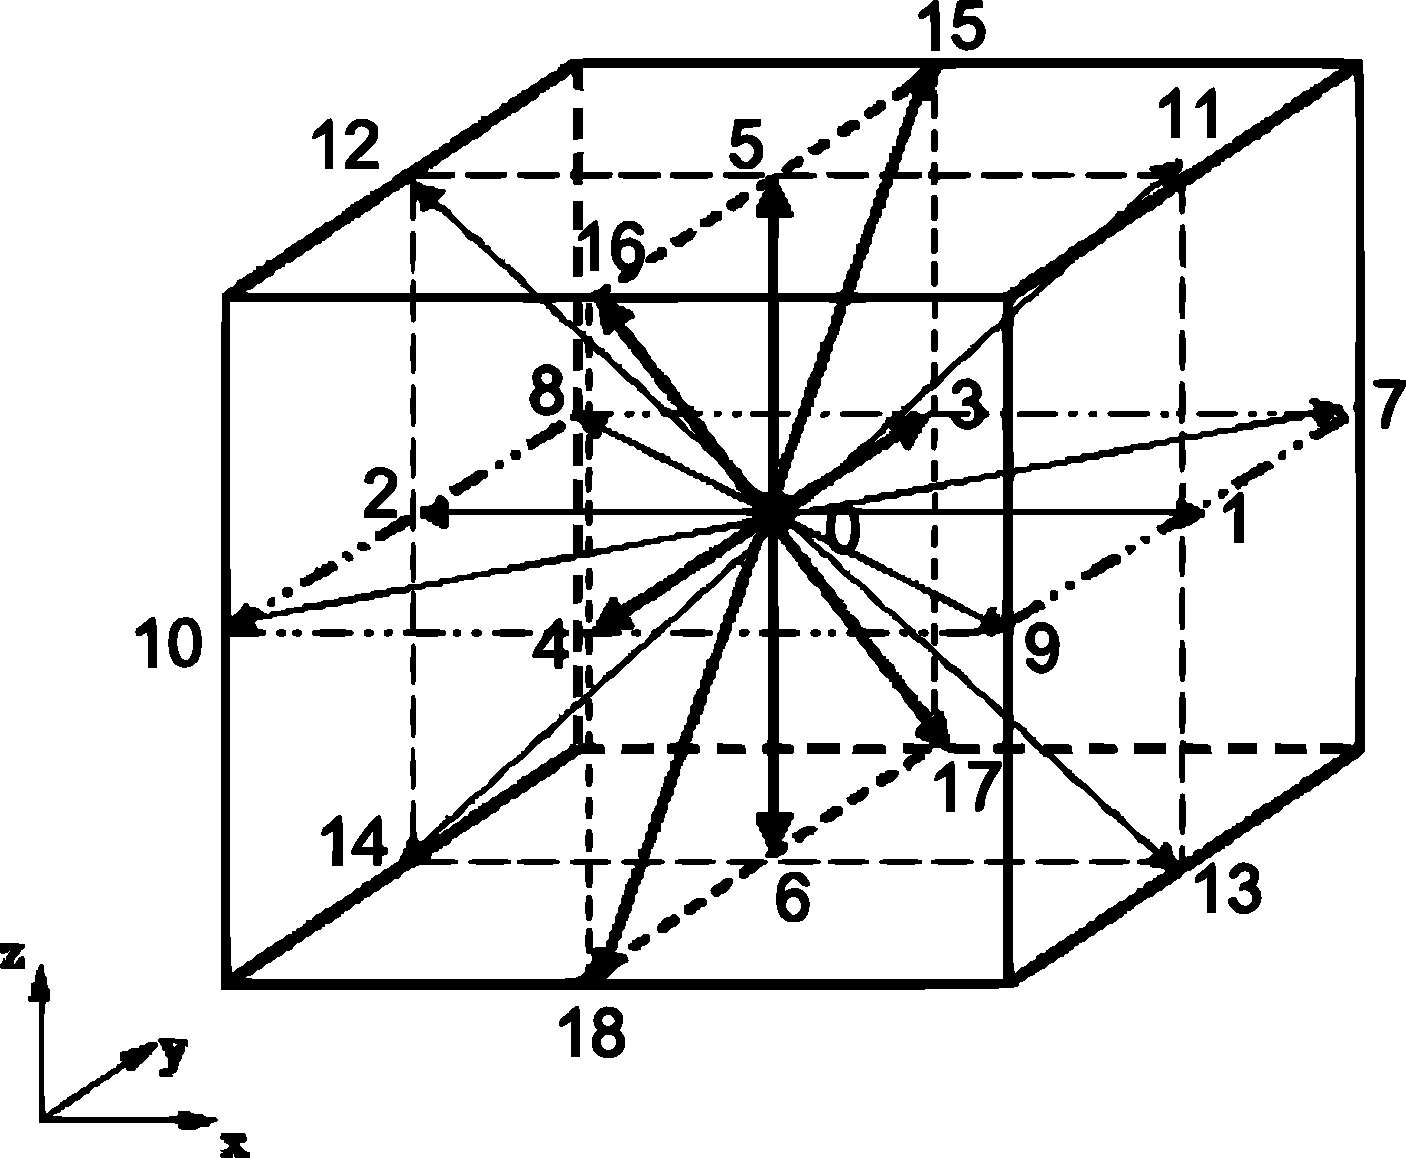
\includegraphics[width=.8\linewidth]{figuras/d3q19.pdf}
  \caption[Esquemático do D3Q19]{Esquemático do modelo D3Q19. Ilustração adaptada do estudo de \citeonline{premnath2013investigation}.}
  \label{fig:d3q19}
\end{figure}

Na Figura \ref{fig:d3q19} é possível visualizar espacialmente as direções de propagação da célula. Vale ressaltar que para cada direção há o cáculo da função de Maxwell ($f_{i}^{M}$) e, por conseguinte, a operação de propagação das funções de distribuição para a célula adjacente no sentido de cada direção.

\subsection{Múltiplos Tempos de Relaxação}

A equação \ref{eq:omega_i} retrata um operador de colisão com tempo de relaxação único. Essa abordagem é funcional porém, em regimes de pouca viscosidade cinemática como é o caso do ar, começa a desenvolver várias instabilidades e divergências como mostra o estudo de \citeonline{lallemand2000theory}. Para esses tipos de problemas a abordagem de múltiplos tempos de relaxação, \textit{multiple}-\textit{relaxation}-\textit{time} (MRT)\abreviatura{MRT}{\textit{multiple}-\textit{relaxation}-\textit{time}}, pode ser usada assim como é mostrado nos estudos de \citeonline{viggen2014lattice}.

De acordo com o esquema proposto por \citeonline{d1994generalized}, a formulação de MRT se baseia na troca do parâmetro de único tempo de relaxação $\tau$ por uma matriz \textbf{$\Lambda$} de vários tempos de relaxação. Todavia a matriz \textbf{$\Lambda$} é construída de acordo com uma matriz \textbf{$M$} que projeta as funções de distribuição $f_{i}$ e $f_{i}^{M}$ no espaço dos momentos. De acordo com \citeonline{lallemand2000theory}, a possibilidade desse método ser mais estável é oriunda da capacidade de operar a colisão das células com um tempo de relaxação apropriado para cada um dos vários momentos, projetados a partir das funções de distribuição $f_{i}$ e $f_{i}^{M}$. Em vista do exposto o operador de colisão da equação \ref{eq:omega_i} se transforma em
\begin{equation}
	\Omega_{i} = -\textbf{$\Lambda$}(f_{i} - f_{i}^{M}).
    \label{eq:MRT_1}
\end{equation}
Porém a operação de colisão é realizada no espeço dos momentos, logo é preciso projetar $f_{i}$ e $f_{i}^{M}$ no espeço dos momentos ficando
\begin{equation}
	m_{i} = \textbf{$M$}f_{i} \text{ e } m_{i}^{M} = \textbf{$M$}f_{i}^{M}.
    \label{eq:MRT_2}
\end{equation}
Considerando que a matriz \textbf{$S$} é dada por
\begin{equation}
	\textbf{$S$} = \textbf{$M$}\textbf{$\Lambda$}\textbf{$M$}^{-1},
    \label{eq:MRT_3}
\end{equation}
o operador de colisão fica
\begin{equation}
	\Omega_{i} = -\textbf{$M$}^{-1}\textbf{$S$}(m_{i} - m_{i}^{M}).
    \label{eq:MRT_4}
\end{equation}
Inserindo a equação \ref{eq:MRT_4} na equação \ref{eq:f_i} fica
\begin{equation}
	f_{i}(\textbf{x} + c_{i}\Delta t, t + \Delta t) = f_{i}(\textbf{x}, t) -\textbf{$M$}^{-1}\textbf{$S$}(m_{i} - m_{i}^{M}).
    \label{eq:MRT_5}
\end{equation}
Vale ressaltar que a operação de propagação, lado esquerdo da equação \ref{eq:MRT_5}, ocorre no espaço original da função de distribuição $f_{i}$.

\subsection{Transformações para Unidades Físicas}

Quando as equações \ref{eq:rho}, \ref{eq:u}, \ref{eq:p} e \ref{eq:nu} são usadas para recuperar os atributos macroscópicos do fluido a unidade de medida não é uma unidade física. Segudo o trabalho de \citeonline{da2016prediction}, para se ter esses atributos em unidade física é preciso aplicar regras de conversão. Essas regras de conversão se baseiam em duas constantes que são definidas a partir de unidades físicas: velocidade característica definida por   
\begin{equation}
	\zeta = c^{*}/c_{s},
    \label{eq:conversao_1}
\end{equation}
tal que $c^{*}$ é a velocidade física do som, e discretização $\Delta x$ definida pela quantidade de metros por tamanho de célula.

Com os parâmetros $c^{*}$ e $\Delta x$ pode-se realizar as seguintes conversões para unidades físicas:
\begin{gather*}
	\textbf{$u^{*}$} = \zeta \textbf{$u$}\text{, } \\ \textbf{$x^{*}$} = \Delta x\textbf{$x$}
	\text{, } \\ t^{*} = \frac{\Delta x}{\zeta}t \text{, } \\ \nu^{*} = \zeta \Delta x \nu
	\text{, } \\ \rho^{*} = \frac{\zeta}{\Delta x} \rho \text{, } \\ p^{*} = p \zeta^{2}  \rho^{*}_{0} \text{ e } \\ f^{*} = f\frac{\zeta}{\Delta x},
    \label{eq:conversao_1}
\end{gather*}
tal que as variáveis assinaladas com $*$ estão em unidades físicas e $f^{*}$ e $f$ são unidades de frequências física e do LBM respectivamente\simbolo{$f^{*}$}{Frequência física}\simbolo{$f$}{Frequência em LBM}.

\subsection{Condições de Contorno}

Como ocorre nas técnicas numéricas tradicionais, o LBM possui também possui condições de contorno. Como mostra o estudo \citeonline{viggen2014lattice}, as condições de contorno para LBM podem ser classificadas em dois tipos: explícita e implícita. As condições de contorno explícitas são aquelas aplicadas em cada célula, tendo a natureza totalmente alinhada entre elas no domínio, normalmente condições como essas são aplicações personalizadas do cálculo do operador de colisão $\Omega_{i}$. As condições de contorno implícitas são aquelas aplicadas numa região do domínio não alinhado entre as células, normalmente essas condições são aplicadas na operação de propagação. A seguir serão apresentadas as condições de contorno abordadas nesse trabalho, cada uma de cada classificação apresentada.

\subsubsection{\textit{Bounceback}}

De acordo com o estudo de \citeonline{viggen2014lattice}, a condição de contorno do tipo \textit{bounceback} tem como objetivo simular uma parede rígida no domínio do LBM, sendo ela do tipo implícita e localizada entre as células. Há dois tipos de \textit{bounceback}: \textit{free-slip}, que simula escorregamento livre do fluido na condição de contorno e \textit{no-slip}, que simula camada limite do fluido na condição de contorno. Nesse trabalho foi usado o do tipo \textit{no-slip} pois num caso real o escoamento desenvolve camada limite na parede rígida.

A condição de contorno \textit{bounceback} \textit{no-slip} é geralmente implementada na etapa de propagação a partir de uma inversão de funções de distribuição de partículas. A Figura \ref{fig:bounceback} mostra um esquemático de exemplo do processo de funcionamento dessa condição de contorno. 

\begin{figure}[ht!]
\centering
  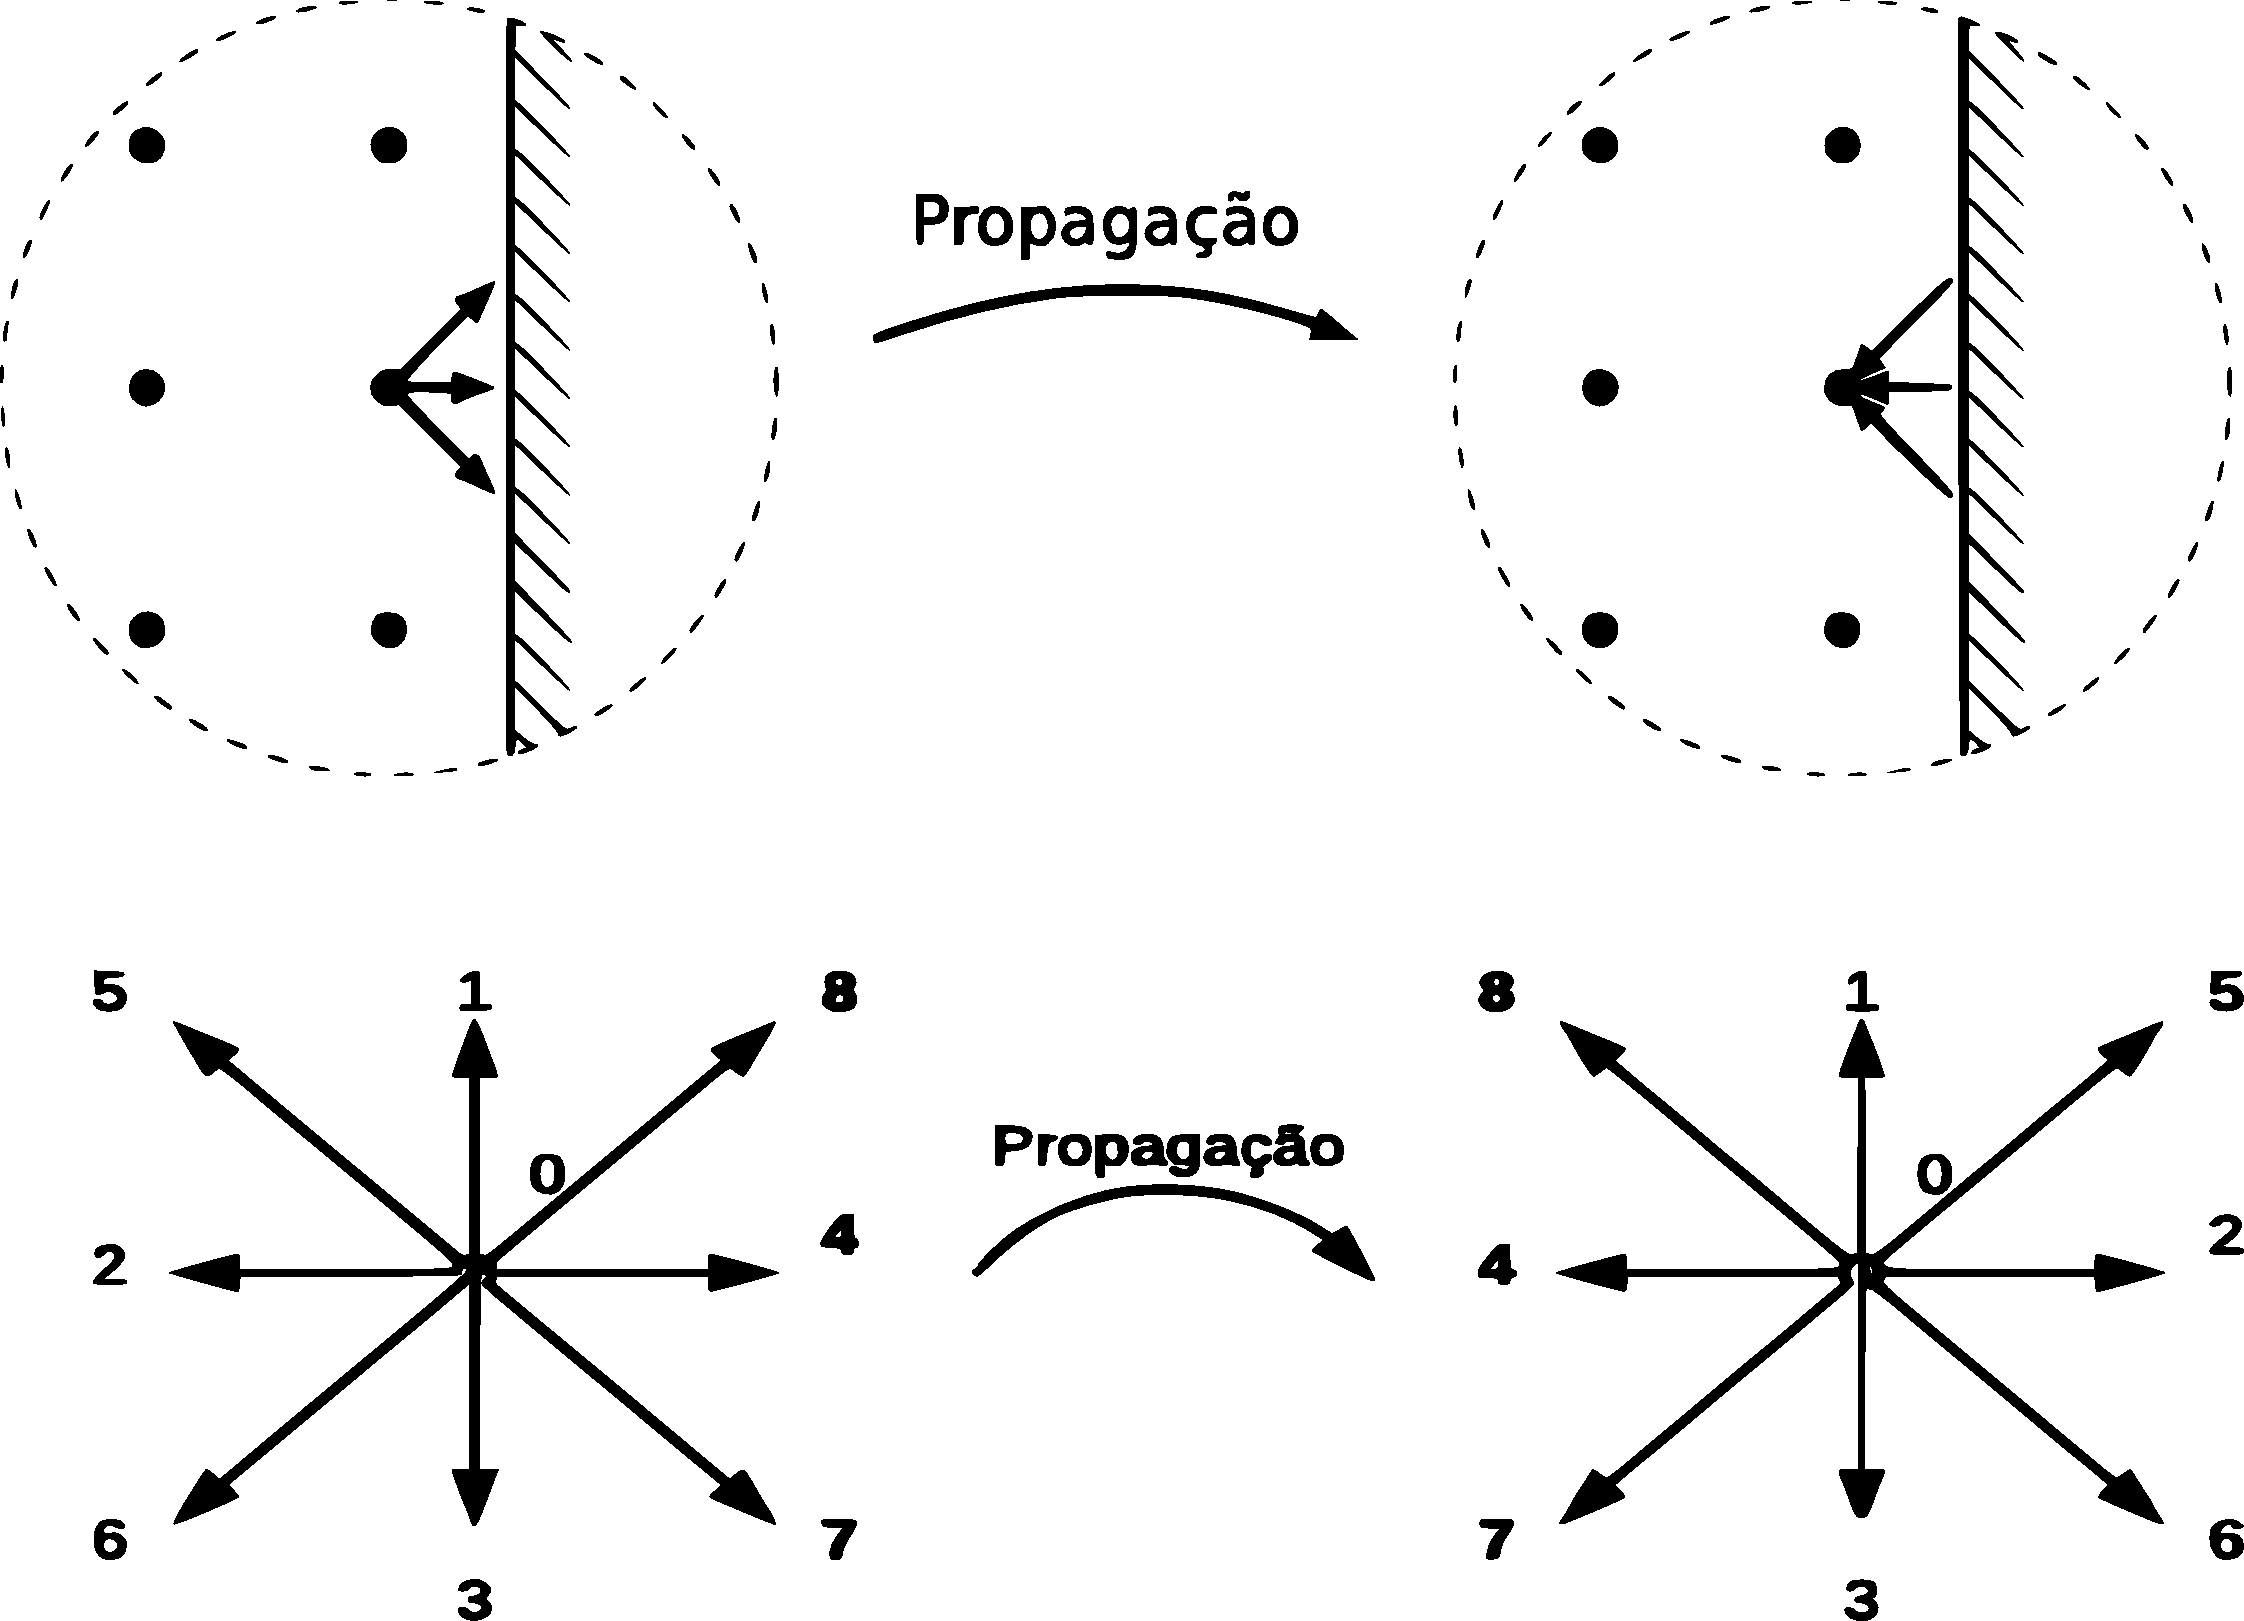
\includegraphics[width=.65\linewidth]{figuras/bounceback.pdf}
  \caption[Processo de funcionamento do \textit{bounceback} \textit{no-slip}]{Esquemático de exemplo do processo de funcionamento da condição de contorno \textit{bounceback} \textit{no-slip}. Ilustração adaptada do estudo de \citeonline{viggen2014lattice}.}
  \label{fig:bounceback}
\end{figure}

De acordo como é mostrado na Figura \ref{fig:bounceback}, ao cruzar a condição de contorno, a célula inverte as funções de distribuição de partículas para o sentido contrário dos vetores que apontam para o \textit{bounceback}. Em relação às equações de propagação o processo abordado fica

\begin{gather*}
  f_{6}(\textbf{x}, t + \Delta t) = f_{8}(\textbf{x}, t)\text{,  } f_{8}(\textbf{x}, t + \Delta t) = f_{6}(\textbf{x}, t), \\
  f_{2}(\textbf{x}, t + \Delta t) = f_{4}(\textbf{x}, t)\text{,  } f_{4}(\textbf{x}, t + \Delta t) = f_{2}(\textbf{x}, t) \text{ e }\\
  f_{5}(\textbf{x}, t + \Delta t) = f_{7}(\textbf{x}, t)\text{,  } f_{7}(\textbf{x}, t + \Delta t) = f_{5}(\textbf{x}, t).
\label{eq:bounceback}
\end{gather*}

\subsubsection{Condição Anecóica}

Consolidar uma condição do tipo anecóica num método numérico de natureza temporal é um desafio. Em vez de ser no domínio do tempo, a propriedade de condição anecóica ou absorção de energia acústica é constituída no domínio da frequência ($Z_{0}$ $=$ $\rho_{0}c_{0}$). Nesse contexto, considerando a absorção de pressão, entropia e pulsos de despredimento de vórtices, o trabalho de \citeonline{kam2006non} propõe uma condição de contorno explícita de absorção. Ela é baseada em técnicas aplicadas na resolução das equações de Navier-Stokes usando DNS (\textit{Direct} \textit{Numerical} \textit{Simulation})\abreviatura{DNS}{\textit{Direct} \textit{Numerical} \textit{Simulation}}. A condição de contorno de absorção, \textit{Absorbing} \textit{Boundary} \textit{Condition} (ABC)\abreviatura{ABC}{\textit{Absorbing} \textit{Boundary} \textit{Condition}}, consiste na adição de uma região de amortecimento para que os valores de pressão e velocidade convirjam assintoticamente a valores que caracterizam um fluido em repouso. Nesse sentido, valores alvos para um fluido em resposo de densidade ($\rho_{T}$ $=$ $\rho_{0}$) e velocidade (\textbf{$u_{T}$} $=$ $0$) são usados para calcular uma função de distribuição de amortecimento $f_{i}^{T}$\simbolo{$f_{i}^{T}$}{Função de distribuição de amortecimento}. Essa função de distribuição é definida da mesma forma que $f_{i}^{M}$, porém com os valores alvos de densidade e velocidade, ficando na forma
\begin{equation}
  f_{i}^{T} = \rho_{0}\varepsilon_{i}.
  \label{eq:f_alvo}
\end{equation}
Como essa técnica é explícita, o operador de colisão $\Omega_{i}$ é adaptado e recebe um novo termo de colisão, ficando na forma
\begin{equation}
  \Omega_{i} = -\frac{1}{\tau}(f_{i} - f_{i}^{M}) - \sigma(f_{i}^{M} - f_{i}^{T}),
  \label{eq:omega_i_abc}
\end{equation}
tal que $\sigma$ $=$ $\sigma_{T}(\delta/D)^{2}$ é o coeficiente de absorção, $\sigma_{T}$ é uma constante com valor de $0,3$, $\delta$ é a distância medida do começo da região de contorno no sentido da convergência assintótica e $D$ é o tamanho total da região de contorno no sentido da convergência assintótica.

O operador de colisão da equação \ref{eq:omega_i_abc} funciona bem para o modelo SRT, porém como nesse estudo será usado o modelo MRT algumas adaptações precisam ser realizadas, pois a operação de colisão ocorre no espaço dos momentos nesse modelo. Assim como é feito nas equações \ref{eq:MRT_2} deve-se aplicar o mesmo procedimento na função de distribuição $f_{i}^{T}$ ficando
\begin{equation}
  m_{i}^{T} = \textbf{$M$}f_{i}^{T}.
  \label{eq:abc_mrt_1}
\end{equation}
Além disso é preciso inserir esse termo no operador de colisão da equação \ref{eq:MRT_4} resultando em 

\begin{equation}
  \Omega_{i} = -\textbf{$M$}^{-1}\textbf{$S$}(m_{i} - m_{i}^{M}) - 
  \sigma\textbf{$M$}^{-1}\textbf{$S$}(m_{i}^{M} - m_{i}^{T}).
  \label{eq:abc_mrt_2}
\end{equation}

Simplificando a equação \ref{eq:abc_mrt_2} fica
\begin{equation}
  \Omega_{i} = -\textbf{$M$}^{-1}\textbf{$S$}[m_{i} - m_{i}^{M}(\sigma - 1) - m_{i}^{T}].
  \label{eq:abc_mrt_3}
\end{equation}

Adicionando esse termo na equação geral \ref{eq:f_i} do LBM o resultado é a equação
\begin{equation}
  f_{i}(\textbf{x} + c_{i}\Delta t, t + \Delta t) = f_{i}(\textbf{x}, t) -\textbf{$M$}^{-1}\textbf{$S$}[m_{i} - m_{i}^{M}(\sigma - 1) - m_{i}^{T}].
  \label{eq:abc_mrt_4}  
\end{equation}

\section{Palabos}

Aliado aos métodos númericos há várias tecnologias computacionais que são essenciais para aplicação e resolução de equações complexas. É bastante comum o uso de \textit{softwares} proprietários para desenvolvimento de modelos numéricos mas os mesmos restringem o desenvolvimento de estudos, ferramentas e produtos científicos. Dos fatores de restrição pode-se destacar:

\begin{itemize}
  \item não é possível saber com exatidão os métodos e equações que estão implementados no \textit{software};
  \item incapacidade do usuário realizar algum tipo de manutenção, correção de defeitos ou evolução no \textit{software};
  \item altos custos de licença de uso. 
\end{itemize}

Em vista das limitações dos \textit{softwares} proprietários, ou seja, projetos de código fechado há outras possibilidades para contornar essas limitações: \textit{softwares} livres. De acordo com \citeonline{stallman2002free} \textit{softwares} livres se caracterizam por cinco liberdades essenciais:

\begin{itemize}
  \item A liberdade de executar o programa como você desejar, para qualquer propósito;
  \item A liberdade de estudar como o programa funciona, e adaptá-lo às suas necessidades. Para tanto, acesso ao código-fonte é um pré-requisito;
  \item A liberdade de estudar como o programa funciona, e adaptá-lo às suas necessidades. Para tanto, acesso ao código-fonte é um pré-requisito;
  \item A liberdade de redistribuir cópias de modo que você possa ajudar ao próximo;
  \item A liberdade de distribuir cópias de suas versões modificadas a outros. Desta forma, você pode dar a toda comunidade a chance de beneficiar de suas mudanças. Para tanto, acesso ao código-fonte é um pré-requisito.
\end{itemize}

Tais liberdades favorecem o desenvolvimento de estudos, ferramentas e produtos científicos com um custo-benefício bastante apropriado para universidades. Considerando isso, projetos de \textit{softwares} livres se tornam atrativos para a implementação dos requisitos do LBM propostos nesse trabalho e, dentro das opções disponíveis no mercado atualmente, o \textit{software} \citeonline{palabos} é classificado como bastante conveniente visto que sua documentação é bastante abrangente, sua arquitetura de \textit{software} é totalmente modularizada com baixo acoplamento e alta coesão e sua tecnologia de processamento chega a ser no mínimo 20 vezes mais rápida que o MATLAB de acordo com \citeonline{numeric_palabos}.   

O \textit{software} livre Palabos é um projeto feito no paradígma computacional de orientação a objetos resultado da colaboração entre indústria e academia, focando produzir uma ferramenta de simulação computacional robusta, rápida e confiável. Todos os modelos nativos são implementados e testados como mostra os estudos de \citeonline{lattice_1}, \citeonline{lattice_2}, \citeonline{lattice_3}, \citeonline{lattice_4} e \citeonline{lattice_5}. De funcionalidades o \textit{software} possui:

\begin{itemize}
  \item dinâmicas físicas:
  \begin{itemize}
     \item equações de Navier-Stokes incompressível e fracamente compressível;
     \item escoamentos com força de corpo;
     \item escoamentos com diferenças de temperatura;
     \item fluidos multifásicos;
     \item modelo de turbulência Smagorinsky.
   \end{itemize}
  \item modelos básicos:
  \begin{itemize}
    \item BGK;
    \item MRT;
    \item entrópico.
  \end{itemize}
  \item condições de contorno:
  \begin{itemize}
    \item \textit{bounceback};
    \item Zou/He;
    \item Inamuro;
    \item Skordos;
    \item periódico;
    \item Dirichlet para velocidade ou pressão.
  \end{itemize}
  \item geração de malha:
  \begin{itemize}
    \item criação de malha a partir de arquivos CAD do tipo STL.  
  \end{itemize}
  \item grid:
  \begin{itemize}
    \item D2Q9;
    \item D3Q13;
    \item D3Q15;
    \item D3Q19;
    \item D3Q27;
    \item \textit{Multi-grid}. 
  \end{itemize}
  \item paralelismo:
  \begin{itemize}
    \item MPI em vários processadores;
    \item MPI em vários computadores em rede.
  \end{itemize}
  \item dados de saída:
  \begin{itemize}
    \item arquivos de dados em ASCII;
    \item arquivos de dados em formato binário;
    \item arquivos de dados em formato de imagem GIF;
    \item arquivos de dados em formato VTK para visualização no \textit{software} \citeonline{paraview}.
  \end{itemize}
\end{itemize}

Mesmo com várias funcionalidades nativas, o \textit{software} \citeonline{palabos} precisa ter outras outras funcionalidades implementadas para que possa atender o escopo desse trabalho. Para atender esse requisito, o projeto \citeonline{palabos_acoustic} foi criado como uma versão do \citeonline{palabos} que contém todos os modelos e implementações desenvolvidas nesse trabalho. As funcionalidades desenvolvidas nesse trabalho são:

\begin{itemize}
  
  \item condições de contorno:
  \begin{itemize}
    \item condição de contorno anecóica de \citeonline{kam2006non} para BGK D2Q9;
    \item condição de contorno anecóica de \citeonline{kam2006non} para MRT D2Q9 e D3Q19;
    \item condição de contorno para excitação do duto com \textit{sweep} ou soma de harmônicos.
  \end{itemize}

  \item geração de malha:
  \begin{itemize}
    \item criação automática de malha com vários tamanhos e espessuras de dutos.
  \end{itemize}

  \item dados de saída:
  \begin{itemize}
    \item relatórios automáticos de execução;
    \item dados e relatórios de execução organizados automaticamente por pastas com hora e data.
  \end{itemize}
\end{itemize}


Para executar o \citeonline{palabos_acoustic} é preciso dos seguintes \textit{softwares} básicos instalados como pré-requisitos:

\begin{itemize}
  \item sistema operacional linux Ubuntu 16.04 ou CentOS 7.2;
  \item compilador de C++ do tipo g++ 4.8;
  \item biblioteca de processamento paralelo Open MPI 1.10. 
\end{itemize}

Para cada novo modelo é preciso criar uma pasta com o nome do modelo contendo o arquivo de compilação \textbf{Makefile} e o código fonte do modelo numérico escrito em C++ com extenção \textbf{.cpp}. No arquivo \textbf{Makefile} é possível configurar aonde se encontra a instalação do Palabos, arquivo do modelo numérico com extenção \textbf{.cpp}, opções de depuração e opções de paralelização. No arquivo de extenção \textbf{.cpp} se encontra o código fonte do modelo numérico a ser simulado e o mesmo é composto de acordo com os procedimentos do fluxograma da Figura \ref{fig:palabos_fluxo}.


\begin{figure}[ht!]
\centering
  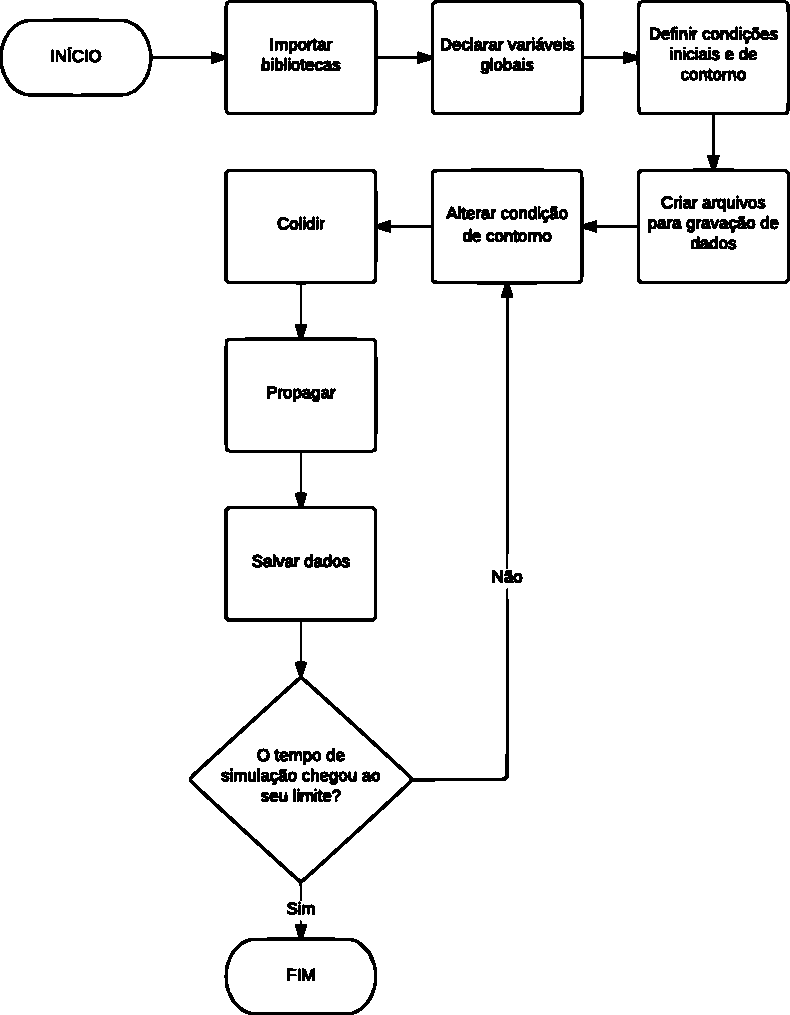
\includegraphics[width=.8\linewidth]{figuras/palabos_modelo_fluxo.pdf}
  \caption[Fluxograma de um modelo numérico no Palabos]{Fluxograma geral de um código fonte de um modelo numérico no Palabos.}
  \label{fig:palabos_fluxo}
\end{figure}

Como é mostrado na Figura \ref{fig:palabos_fluxo}, todo código de modelo numérico no Palabos possui os seguintes procedimentos:

\begin{itemize}
  \item importar bibliotecas: nesse procedimento são importadas as bibliotecas que contêm as funções e classes que serão usadas ao longo do processamento do modelo. Normalmente são bibliotecas do próprio Palabos ou bibliotecas com funções matemáticas;
  \item definir variáveis globais: normalmente nessa etapa são definidas valores de pré-processamento como o tamanho do domínio, valores macroscópicos do fluido como número de Reynolds, tempo total de simulação, viscosidade cinemática e o tipo de modelo LBM;
  \item definir condições iniciais e de contorno: nessa etapa a malha do domínio é consolidada, valores de densidade e velocidade são atribuídas para cada célula do domínio e condições de contorno são impostas;
  \item criar arquivos para gravação de dados: são criados ponteiros e arquivos de diversas extensões para que os dados sejam gravados;
  \item alterar condição de contorno: nessa etapa o modelo numérico entra no \textit{loop} de iterações e se necessário as condições de contorno são alteradas para, por exemplo, que um \textit{sweep} possa ser imposto;
  \item colidir: nessa etapa o operador de colisão é calculado e somado com as funções de distribuição de cada célula;
  \item propagar: os valores das funções de distribuição são propagados para células vizinhas;
  \item salvar dados: os dados normalmente de pressão e velocidades são salvos para pós-processamento. 
\end{itemize}
E assim o ciclo de procedimentos dentro do \textit{loop} é executado até que o número de iterações alcance o número máximo de tempo definido no início do programa.

Para execução é preciso efetuar os seguintes comandos no terminal linux dentro da pasta do modelo numérico:
\begin{itemize}
  \item compilação do código de extenção \textbf{.cpp} para formato binário em linguagem de máquina:
  \begin{lstlisting}[language=make, frame = single]
    $ make
  \end{lstlisting}
  \item execução do arquivo binário compilado:
  \begin{lstlisting}[language=make, frame = single]
    $ mpirun -np 
    <numero_de_processadores> 
    <nome_do_arquivo_compilado> 
    <parametros_de_entrada>
  \end{lstlisting}
  aplicando para o modelo numérico desse trabalho:
  \begin{lstlisting}[language=make, frame = single]
    $ mpirun -np 
    8
    duct_radiation_optimization
    20 0.15 1.99
  \end{lstlisting}
  tal que o raio do duto é 20 células, o mach do escoamento é 0.15 e 1.99 é a frequência de relaxação $1/\tau$. É possível também executar o Palabos com o \textit{script} \textbf{duct\_radiation\_init.m} na plataforma \citeonline{matlab} ou \citeonline{octave}. Para executar basta colocar esse \textit{script} dentro da pasta do modelo numérico e executar o seguinte comando no terminal do \citeonline{matlab} ou \citeonline{octave} dentro dessa pasta:
  \begin{lstlisting}[language=matlab, frame = single]
    >> duct_radiation_init 20 0.15 5042 8
  \end{lstlisting}
  tal que o raio do duto é 20 células, o mach do escoamento é 0.15, o número de Reynolds é 5042 e o 8 é a quantidade de processadores.
\end{itemize}


\section{Modelo Numérico}

Com os arquivos de compilação e execução corretamente configurados, pode-se modelar numericamente o problema. A Figura \ref{fig:modelo} representa a vista do corte lateral do modelo numérico em 3D. Para a definição do domínio foi utilizado uma abordagem paramétrica, ou seja, o raio externo do duto $a$ $=$ $20$ células foi a unidade de medida para as dimensões. As dimensões \textbf{Nx} e \textbf{Ny} são iguais e possuem $20a$ de comprimento. A dimensão \textbf{Nz} possui 79,5$a$ de comprimento e foi baseada no estudo de \citeonline{allam2006investigation}, que justifica a distância da saída do duto até a parede para minimizar os efeitos da interação do jato de saída com a parede. Todo espaço de fluido do domínio foi preenchido em cada célula com frequência de relaxação $\frac{1}{\tau}$ $=$ $1,99$, $\rho$ $=$ $\rho_{0}$ $=$ $1$ e as velocidades para todos os sentidos $u_{x}$ $=$ $u_{y}$ $=$ $u_{z}$ $=$ $0$. As bordas do duto foram preenchidas com condição anecóica de espessura igual 1,5$a$ células.      

Com relação ao duto, o mesmo possui o tamanho \textbf{L} $=$ $18a$ e é delimitado pela condição de contorno \textit{bounceback} \textit{no-slip}, diâmetro externo medindo $2a$ e parede com expessura de 0,1$a$. No começo do duto há uma condição anecóica com espessura igual a 1,5$a$, que é responsável pela dissipação da onda no sentido contrário a saída. Ao lado da condição anecóica há uma condição de contorno de excitação do duto com espessura de 0,05$a$, responsável por excitar os modos axiais e impor escoamento.    

% \begin{figure}[ht!]
%   \centering
%   \def\svgwidth{400pt}
%   \import{figuras/}{modelo_numerico.pdf_tex}
%   \caption[Esquemático do modelo numérico]{Esquemático do modelo numérico: vista do corte lateral do modelo em 3D.}
%   \label{fig:modelo}
% \end{figure}

\begin{figure}[ht!]
\centering
  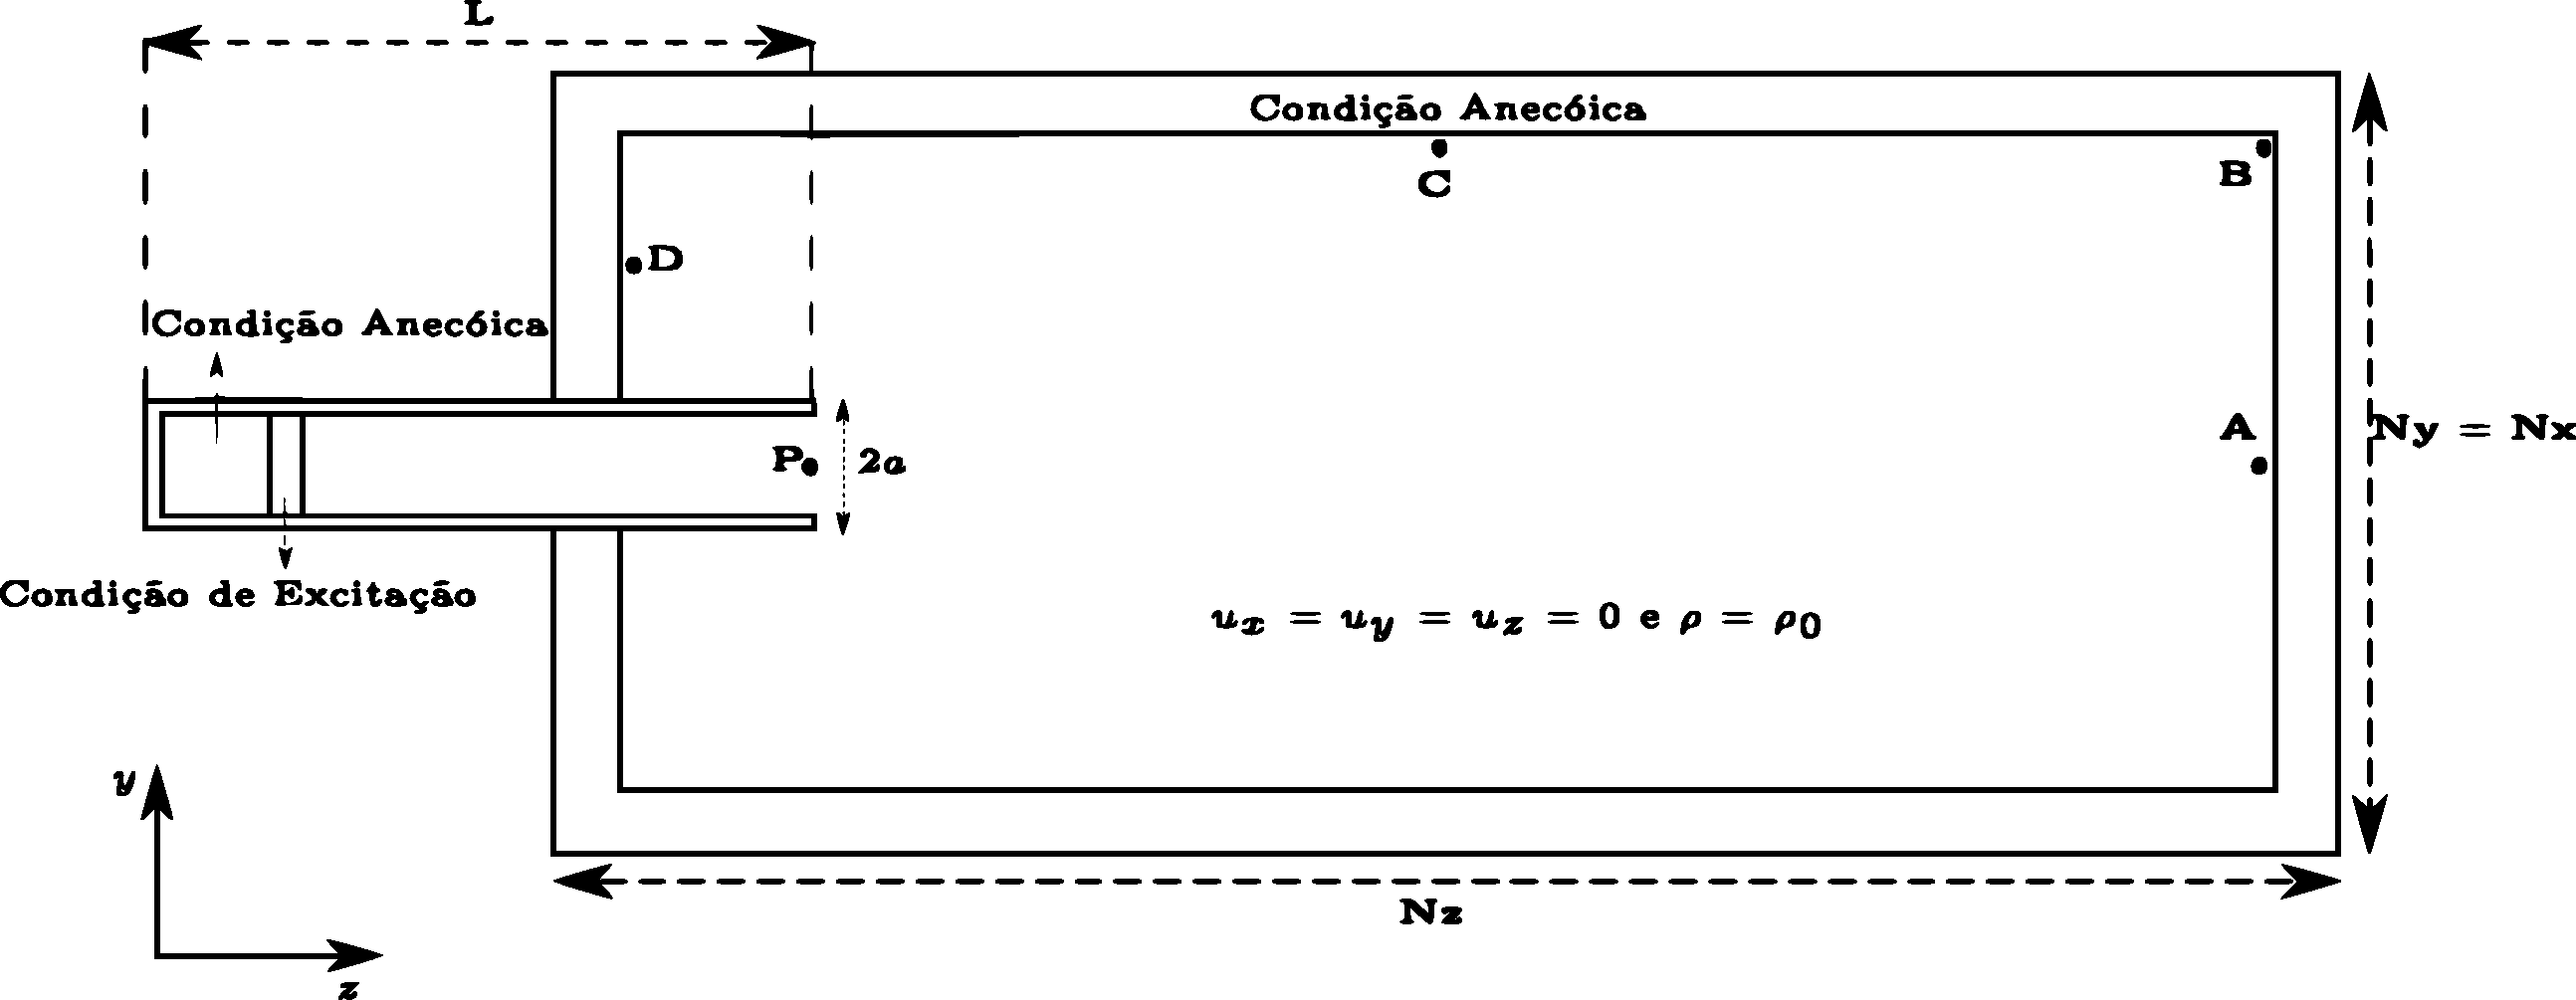
\includegraphics[width=1.\linewidth]{figuras/modelo_numerico_2.pdf}
  \caption[Esquemático do modelo numérico]{Esquemático do modelo numérico: vista do corte lateral do modelo em 3D.}
  \label{fig:modelo}
\end{figure}


Focando propiciar energia suficiente nos modos axiais com onda plana, a condição de excitação foi desenvolvida através de uma soma de ondas estacionárias, na faixa de frequência $0$ $<$ $ka$ $\leq$ 2,5. Dessa forma, os valores de densidade e velocidade dessa região foram mudados em cada incremento de tempo da seguinte forma para:
\begin{itemize}
  \item regime transiente ($0 \leq t < t_{transiente}$):
  \begin{gather*}
    \rho(t) = \rho_{0};% + A\sum_{n=1}^{N} sin\bigg(\frac{nka_{max}c_{s}t}{Na}\bigg);
    \\ u_{z}(t) = Mc_{s};    
    \\ u_{y}(t) = 0;
    \\ u_{x}(t) = 0.
  \label{eq:transiente}
  \end{gather*}

  \item regime estacionário ($t_{transiente} \leq t \leq t_{total} - t_{propagada}$):
  \begin{gather*}
    \rho(t) = \rho_{0} + A\sum_{n=1}^{N} sin\bigg(\frac{nka_{max}c_{s}t}{Na}\bigg);
    \\ u_{z}(t) = Mc_{s} + \frac{Ac_{s}}{\rho_{0}}\sum_{n=1}^{N} sin\bigg(\frac{nka_{max}c_{s}t}{Na}\bigg);    
    \\ u_{y}(t) = 0;
    \\ u_{x}(t) = 0.
  \label{eq:estacionario}
  \end{gather*}
\end{itemize}
tal que $ka_{max} =$ 2,5, $N$ é o número total de ondas estacionárias dentro do intervalo $0$ $<$ $ka$ $\leq$ 2,5, $n$ é uma onda estacionária pertencente a esse mesmo intervalo de frequências, $t_{transiente}$ é baseado e adaptado do estudo de \citeonline{shi2013lattice} na forma $t_{transiente} =  2\textbf{Nz}/Mc_{s}$, $t_{propagada}$ é definido como $t_{propagada} = \textbf{Nz}/c_{s}$ e é o tempo que a onda demora para percorrer o domínio completo na direção axial do duto, $t_{total} = t_{transiente} + t_{propagada} + 12000$ é o tempo total da simulação e $A$ é amplitude máxima definida como densidade e é calculada a partir de uma pressão física na forma
\begin{equation}
  A = \frac{2 \cdot 10^{-5} \cdot 10^{\text{NPS}/20}}{c^{*}\rho^{*}_{0}c_{s}},
\end{equation}
tal que $c^{*} = 343$ $m/s$ é a velocidade do som em unidades físicas, $\rho^{*}_{0} =$ 1,22 $kg/m^{3}$ é a densidade física do ar em unidades físicas e NPS é o nível de pressão sonora no valor de 80 dB.

No intuito de avaliar a condição anecóica nas fronteiras do domínio através do cálculo e análise do coeficiente de reflexão, os pontos $\textbf{A}$, $\textbf{B}$, $\textbf{C}$ e $\textbf{D}$ representados na Figura \ref{fig:modelo} são pontos de medição de pressão e velocidades uma célula ao lado das condições anecóicas. O localização dos pontos segue as seguintes coordenadas:

\begin{itemize}
  \item ponto $\textbf{A}$: $(\frac{\textbf{Nx}}{2}, \frac{\textbf{Ny}}{2}, \textbf{Nz} - 31)$;
  \item ponto $\textbf{B}$: $(\frac{\textbf{Nx}}{2}, \textbf{Ny} - 31, \textbf{Nz} - 31)$;
  \item ponto $\textbf{C}$: $(\frac{\textbf{Nx}}{2}, \textbf{Ny} - 31, \frac{\textbf{Nz}}{2})$;
   \item ponto $\textbf{D}$: $(\frac{\textbf{Nx}}{2}, \frac{3\textbf{Ny}}{4}, 12a + 31)$.
\end{itemize}
 
Já o ponto $\textbf{P}$ representa a média espacial, feita no plano transversal do duto, dos valores de pressão e velocidade na terminação. Essas médias espaciais são extraídas e calculadas ao longo do tempo para se obter os parâmetros de caracterização da acústica interna do duto: coeficiente de reflexão $R_{r}$ e coeficiente de correção da terminação $l/a$.

Para a execução do modelo numérico foi escolhido um \textit{hardware} com as seguintes características:

\begin{itemize}
  \item arquitetura: x86\_64;
  \item CPU(s): 8;
  \item modelo do processador: Intel(R) Xeon(R) CPU E5620 @2.40GHz;
  \item memória RAM: 139 GB.
\end{itemize}

%\newcommand{\MyNumberA}{30}

%\newcommand{\MyNumberB}{60}

%\MyNumberB

%\numexpr (\MyNumberA + 2* \MyNumberN)/3 \relax
%\the\numexpr (\MyNumberA * \MyNumberB)

\section{Pós-processamento}

Com os arquivos de dados temporais dos pontos $\textbf{A}$, $\textbf{B}$, $\textbf{C}$, $\textbf{D}$ e da média espacial $\textbf{P}$ salvos em disco rígido, um \textit{script} de pós-processamento da plataforma \citeonline{matlab}/\citeonline{octave} é executado. Os seguintes procedimentos são realizados no \textit{script}:

\begin{enumerate}
  \item os vetores temporais de pressão e velocidade no eixo axial são obtidos através da leitura de arquivos \textbf{.dat};
  \item uma janela Hann na forma
  \begin{equation}
    w(n) = sin^{2}\bigg(\frac{\pi n}{N - 1} \bigg),  
  \end{equation}
  tal que $N$ é o tamanho da janela e $n$ é a posição do vetor unidimensional é definida e usada para multiplar os sinais de velocidade e pressão no domínio do tempo;

  \item a transformada rápida de Fourier, \textit{Fast} \textit{Fourier} \textit{Transform} (FFT)\abreviatura{FFT}{\textit{Fast} \textit{Fourier} \textit{Transform}}, é aplicada nos vetores de velocidade e pressão no domínio do tempo;

  \item a impedância de radiação $Z_{r}$ é calculada através da divisão entre os vetores de pressões por de velocidades no domínio da frequência da seguinte forma:
  \begin{equation}
    Z_{r} = \frac{p(f)}{u_{z}(f)};
  \end{equation}

  \item o coeficiente de reflexão $R_{r}$ é calculado de acordo com a equação \ref{eq:R};

  \item o coeficiente de correção da terminação $l/a$ é calculado de acordo com a equação \ref{eq:l};

 \end{enumerate}

 Para minimizar os efeitos não lineares de ondas evanescentes na terminação do duto, um fator de correção $c = - 0,2367$ é adicionado na parte real do coeficiente de correção da terminação $l/a$.    